%% =============================== PREAMBLE ====================================

\documentclass[conference]{IEEEtran}

\usepackage{cite,amsmath,amssymb,amsfonts,algorithmic,graphicx,textcomp,xcolor,
  etoolbox}

\pdfminorversion=7
\pdfsuppresswarningpagegroup=1
\IEEEoverridecommandlockouts
\apptocmd{\sloppy}{\hbadness 10000\relax}{}{}
\def\BibTeX{{\rm B\kern-.05em{\sc i\kern-.025em b}\kern-.08em
    T\kern-.1667em\lower.7ex\hbox{E}\kern-.125emX}}

\newcommand{\project}{{\sc{Collaborate}}~}
\newcommand{\cpp}{C\texttt{++}~}
%\newcommand{\thisplace}{\textit{Department of Electrical}\\
%  \textit{and Computer Engineering}\\
%  \textit{The Ohio State University}\\
%  Columbus OH, USA\\
%}
\newcommand{\thisplace}{\ \ {Dept. Elec. \& Comp. Eng.}\ \ \\
  {The Ohio State University}\\
  Columbus, OH, USA\\
}

\title{Using Cognitive Communications to Increase the Operational Value of
  Collaborative Networks of Satellites}

 \author{
   \IEEEauthorblockN{Ryan B. Linnabary}
   \IEEEauthorblockA{\thisplace linnabary.24@osu.edu}
   \and
   \IEEEauthorblockN{Andrew J. O'Brien}
   \IEEEauthorblockA{\thisplace obrien.200@osu.edu}
   \and
   \IEEEauthorblockN{Graeme E. Smith}
   \IEEEauthorblockA{\thisplace smith.8347@osu.edu}
   \and
   \IEEEauthorblockN{Christopher Ball}
   \IEEEauthorblockA{\thisplace ball.51@osu.edu}
   \and {~} \and {~~~~~~~~~~~~~~~~} \and
   \IEEEauthorblockN{Joel T. Johnson}
   \IEEEauthorblockA{\thisplace johnson.1374@osu.edu}
   \and {~~~~~~} \and {~~~~~~}
 }
%\author{
%  \IEEEauthorblockN{Ryan B. Linnabary}
%  \IEEEauthorblockA{\thisplace linnabary.24@osu.edu}
%  \and
%  \IEEEauthorblockN{Andrew J. O'Brien}
%  \IEEEauthorblockA{\thisplace obrien.200@osu.edu}
%  \and
%  \IEEEauthorblockN{Graeme E. Smith}
%  \IEEEauthorblockA{\thisplace smith.8347@osu.edu}
%  \and {~} \and {~~~~~~~~~~~~~~~} \and
%  \IEEEauthorblockN{Christopher Ball}
%  \IEEEauthorblockA{\thisplace ball.51@osu.edu}
%  \and {~~~~~~~~~~~~~~~} \and
%  \IEEEauthorblockN{Joel T. Johnson}
%  \IEEEauthorblockA{\thisplace johnson.1374@osu.edu}
%  \and {~~~~~~~~~~~~~~~}
%}

%% =============================== DOCUMENT ====================================

\begin{document}

\maketitle

\IEEEpubid{
  \begin{minipage}{\textwidth}
    {
      %TODO:  AJO: this needs to be above the bottom margin, unfortunately.  But not sure how 
      % to force the column text to break early 
      \ \\ \\ \\ \\ \\ [12pt]
      \rule{0.49\textwidth}{0.4pt} \\
      \hphantom{10pt}This research was sponsored by the NASA Advanced
      Information Sys-\\tems Technology Program NNH16ZDA001N-AIST. \\
      %\\
      %\normalsize
      %978-1-7281-0048-7/19/\$31.00 \copyright2019 IEEE
    }
  \end{minipage}
}

%% =============================== ABSTRACT ====================================

\begin{abstract}
Distributed satellite constellations utilizing networks of small satellites will be a key enabler of new observing strategies in the next generation of NASA missions.  While it is quickly becoming feasible to establish communication networks among small satellites, a key question is how these networks can be best utilized to achieve objectives.  While small satellite instruments are becoming more capable, they are still resource constrained (i.e. power, data, scanning systems, etc.); therefore, adaptive instruments that intelligently adjust parameters on the fly are key for increasing operational value within these constraints.  In this context, the purpose of collaborative communication among small satellites is to achieve system-level adaptivity.  This dramatically increases the complexity of the control algorithms and decision space in which the small satellites communication networks must operate.  We postulate that cognition in the high-level collaborative communication is one approach to both achieve autonomy and to address this complex control space.  In this paper, we investigate concepts for how machine learning (ML) algorithms can be utilized in the high-level decision making of a communication system in a distributed satellite mission.  This paper will show cognitive communication model with ML and some example case study results.
\end{abstract}

\begin{IEEEkeywords}
Distributed Satellite Missions, Autonomous Systems, Sensor Network, Sensor Web, OSSE
\end{IEEEkeywords}

%% ============================= INTRODUCTION ==================================

\section{Introduction}
\label{sec:intro}

It is envisioned that NASA's future space systems will be composed of large,
inhomogeneous networks of small satellites and autonomous platforms \cite{ref1}.  These
resource constrained systems, carrying an array of different instruments, will
be expected to operate autonomously and collaboratively to achieve mission and
science goals.  Unfortunately, current and near-future inter-satellite
communications are highly constrained in terms of link availability,
reliability, power and bandwidth.  Although future technologies (such as free
space optical links) may alleviate some constraints, it is expected that future
instruments will rapidly expand in both data volume and sensor
reconfigurability \cite{ref2}.  In this way, it is not sufficient to simply increase the
capabilities of the communication links.  Rather, it is also necessary to
improve the complex decision making that communication systems perform, such as
deciding when to transmit, what information is valuable to nodes of the network,
and how to adapt local operations following the reception of new information.

Recently, cognitive space communication algorithms have been proposed as a
solution to address the complexity of future inter-satellite communication
systems \cite{ref3}.  Typically, these cognitive algorithms have tried to address
communications at a low level and include decision making regarding modulation,
power and bandwidth, and error rate \cite{ref4,ref5}.  However, it is reasonable to expect that
cognition may also offer an improvement in the complex, higher level decisions
of communication in the context of mission and science objectives.  At this
level, cognition is applied to the operation of the network with the decision
making primarily influenced by the constraints of the space communication
network links.

In this work, we show results of simulation studies to explore the advantages
that cognition could offer for collaborative small-satellite networks.  Under a
NASA Advanced Information System Technology program, we are currently developing
an open-source \cpp library for the simulation of autonomous and collaborative
networks of adaptive sensors \cite{ref6}.  This library and accompanying utilities allow for
the efficient simulation of networks of satellites with realistic constraints in
communication, power, and measurements.  A key focus of this software is the
simulation of sensors that operate adaptively.  Adaptive sensors must make
intelligent decisions regarding their configuration based on their own
measurements as well as the measurements provided by other sensors in a network.
However, the extreme complexity of the decision space makes the development of
optimal decision-making systems very difficult.  Thus, an approach based on
cognition could offer an appealing solution.  We investigate how our simulation
tools could be useful for production of large training datasets that capture the
operation of collaborative, adaptive networks of small satellites.  We then
investigate how such a dataset could be combined with machine learning
techniques to train neural networks that could make intelligent decisions about
when and what to communicate.  Results from our investigation will be presented,
and the applicability of these methods to future cognitive space communication
will be discussed.

%% =============================== OVERVIEW ====================================

\section{Collaborative Networks Of Adaptive Sensors}
\label{sec:overview}

{ \color{red}  Satellite sensor constellations are now feasible.  Current constellations are managed in simple ways with ground contacts.  Future constellations operate more autonomously with inter-sat communicaitons}

The remote sensing community anticipates significant demand for simulation tools
as low earth orbit (LEO) small satellites become a common platform for observing
system missions.  This research team has been tasked with developing simulation
tools capable of addressing the challenging problems discussed in
Section~\ref{sec:intro}.  The proposed solution has three main components:
resource management, adaptive sensor hardware, and collaborative networking.
These components may be combined to produce high-fidelity simulations for
validating adaptive sensor designs.

{ \color{red}   Satellites will carry adaptive sensors.  Require ability to make decisions about how to adjust sensor parameters based on own measurements.  more complex to adjust parameters based on entire constelations}

Adaptive sensor networks work together in the following way: a sensor obtains a
measurement, quantifies the measurement's science value and system resource
cost, predicts the network state and data model, and shares this information
with network members.  Network members adapt their behavior or sensor hardware
in response to this new information.  The development process has revealed
opportunities for expansion and improvement involving cognitive communication
and machine learning.

{ \color{red}  Collaboration between satellites enables full utilization of adaptivity.  represents the highest complexity of sensor network.  low TRL.  Difficult to grasp due to complexity.  decision making, reacting to environment and very large space of information.  Can cognition be applied here? }

%% ========================= HIGH-LEVEL COGNITION ==============================

\section{Cognition and High-Level Communications} \label{sec:hlc}

\subsection{Cognitive Communications}
\label{ssec:cognit}
Since many interpretations exist, we begin with defining what is meant by Cognitive Communications.  \textit{Cognition} refers to the act of selecting and carrying out actions based on both specific goals and perception of an external environment.  Cognition necessarily includes learning from past experiences and interactions with the environment.  Thus, a \textit{cognitive entity} is capable of taking action based on its goals and perception of the environment, potentially learning from the result of its action.  It is an intelligent entity that posesses perception, learning, reasoning, and making decisions \cite{x}. \textit{Cognitive Communications} are communications whose operations are in some way dependent on cognition.    

Thus far, research into cognitive communication for satellite systems has been predominantly focuses on low-level communication aspects.  {\color{red} (Insert references and descriptions of conference papers from past CCAA)}.  However, cognition can also be applied to the higher-level aspects of a communication system.  For example, cognition could be applied to the intelligent routing of information within an autonomous satellite sensor network \cite{x}.  Alternatively, this routing could establish a collaborative improvement in mission science return and achieve, in effect, a system level adaptivity in response to events.  Thus, consideration of collaboration to `"adaptive remote sensing'" and feedback are added to traditional inter-satellite communication.

{\color{red} (Summary of different methods for dealing with this problem. Can ML help?)}

\subsection{Machine Learning and Cognitive Communications}
\label{ssec:ml}

Machine learning provides computers the ability to learn without being
explicitly programmed.  Such intelligent machines are capable of accurately
predicting and classifying new data.  Computers can be programmed to learn
autonomously with or without supervision, and often require significant
quantities of training data and careful adjustment of model parameters.  These
techniques are useful for the problems which: require many manual adjustments or
long lists of rules; operate in a fluctuating environment; need to process a
large amount of data; or have no known optimal solution.

Machine learning techniques are currently being applied in the development of
adaptive hardware, resource optimization, and other areas of sensor network
design.  An opportunity exists to use machine learning to optimize information
flow within a collaborative network of satellites.  Improvements would increase
communications efficiency by increasing the value of data contents and reducing
operational resource consumption.

All of the common machine learning algorithms apply to optimization of
high-level communication parameters.  Regression tasks enable satellites to
autonomously adjust parameters for communication, sensing, and on-board data
processing.  Classification of network nodes based on proximity and capabilities
could increase efficiency by informing antenna direction or temporal scheduling.
This research involves the application of new and existing machine learning
algorithms.  Existing algorithms are widely available as third-party Python
modules, and will be discussed later in Section~\ref{sec:software}.  Custom
algorithms are developed for the \cpp library.

% \begin{figure}[t]
%   \centerline{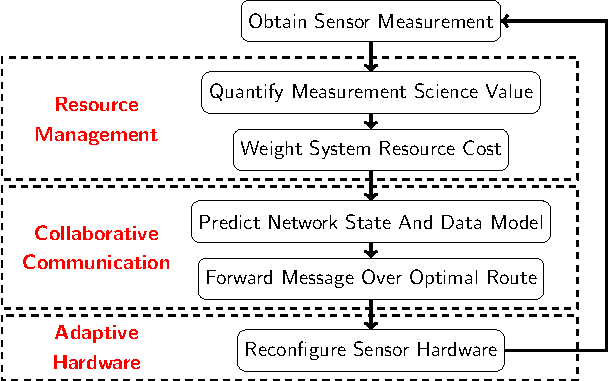
\includegraphics[width=0.75\linewidth]{images/flowchart.pdf}}
%   \caption{Collaborative Model for Adaptive Sensors}
%   \label{fig:model}
% \end{figure}

%\begin{table}[t]
%  \caption{Low vs. high level communication issues}
%  \begin{center}
%    \begin{tabular}{|l|l|}
%      \hline
%      \textbf{Low Level} & \textbf{High Level}\\
%      \hline
%      Bandwidth & Scheduling\\
%      \hline
%      Error Rate & Packet Contents\\
%      \hline
%      Latency & Satellite Health\\
%      \hline
%    \end{tabular}
%    \label{tab:comms}
%  \end{center}
%\end{table}

%\subsection{Cognitive Communications}
%\label{ssec:cognit}

{
  \color{red}
  - Example references of how it has been applied

  - Generation of training data, training of the NN, application of the NN to
  the system. What are input and outputs. What are the steps? List of steps in
  proposed procedure if needed
}

\begin{figure}[t]
  \centerline{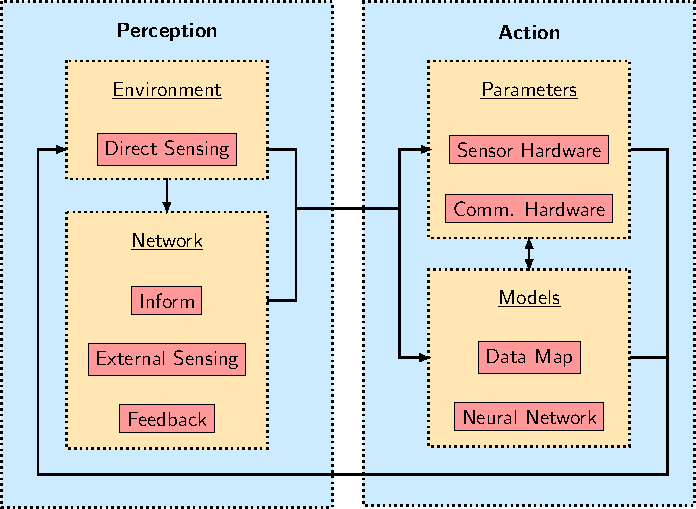
\includegraphics[width=0.9\linewidth]{images/working/flowchart.pdf}}
  \caption{Cognitive Communications Model}
  \label{fig:model}
\end{figure}

\vfill

%% =============================== SOFTWARE ====================================

\section{Sensor Network Simulations to Support Machine Learning Research}
\label{sec:software}

Research in applying machine learning to sensor networks will rely on
simulations to validate algorithms both deployed on spacecraft and on the
ground.  Simulations must provide the means for basic cognitive communication as
well as the production of training data for post-processing by neural networks.
Training data should include simulation variables which are suspected of
correlation to the parameter being optimized.  Variables may capture time-series
data involving satellite position, health, communication hardware details,
sensor hardware details, network connectivity, or other similar parameters.

A software tool-set \project is under development which is capable of producing
the described training data.  The toolset has two main components: first, a \cpp
development library for observing system simulation experiments; and second, a
Python visualization and analysis package for post-processing of data.  The
project is published to a Git repository under the GPLv3.0 license.

The \project library offers a number of unique features valuable to future
observing system simulation experiments.  At its core, it is a physics engine
for satellite position, velocity, and attitude.  Power and RF accessories may be
attached to satellites and individually oriented.  The next level involves rapid
constellation design.  Standard orbit models described by two-line-element (TLE)
sets are provided, copied, and modified to generate novel and interesting
constellation patterns.  Examples are illustrated in Fig.1(a).

Sensor hardware is attached to satellites as an interface to truth data (NetCDF
Nature Run data).  This provides a custom modeling environment for real sensor
hardware and enables heterogeneous sensor constellations with different
capabilities.  As a satellite orbits, its pointing vector intersects Earth's
surface or an atmospheric layer and samples the underlying data, as shown in
Fig.1(b-d).

\project is named for its ability to manage collaborative networks of
satellites.  Its implementation focuses on the high-level communication decision
space previously discussed.  The library employs, in addition to standard \cpp
components, advanced data structures including trees and graphs to execute
predictive route-finding algorithms for efficient communications.  For example,
line-of-sight wireless channels are captured in a graph, as illustrated in
Fig.1(e), the minimum spanning tree.

A predictive scheduling algorithm is illustrated in Fig.1(f).  Satellite ``A''
measures cloud depth in the Pacific Ocean (blue line).  It then predicts the
arrival of a follow-up satellite and relays a message through satellites ``B''
and ``C'' to queue ``D'' for a measurement with a different sensor (red line).
Significant work has been done to optimize this algorithm, because it is the
main consumer of CPU time and is run regularly in simulation to find routes.  It
is also the foundation for deployed cognitive communications, as discussed in
Section~\ref{sec:examples}.

Presently, the included algorithms are iterative and often take minutes to
conclude.  It may be possible to reduce run-time or optimize routes based on
alternative parameters using machine learning.  An option is to replace these
algorithms with predictive neural networks for advanced regression or
classification algorithms.  \project facilitates this by producing data
in standard formats for post-processing.

\begin{figure}[b!]
  \begin{minipage}[b]{\linewidth}
    \begin{center}
      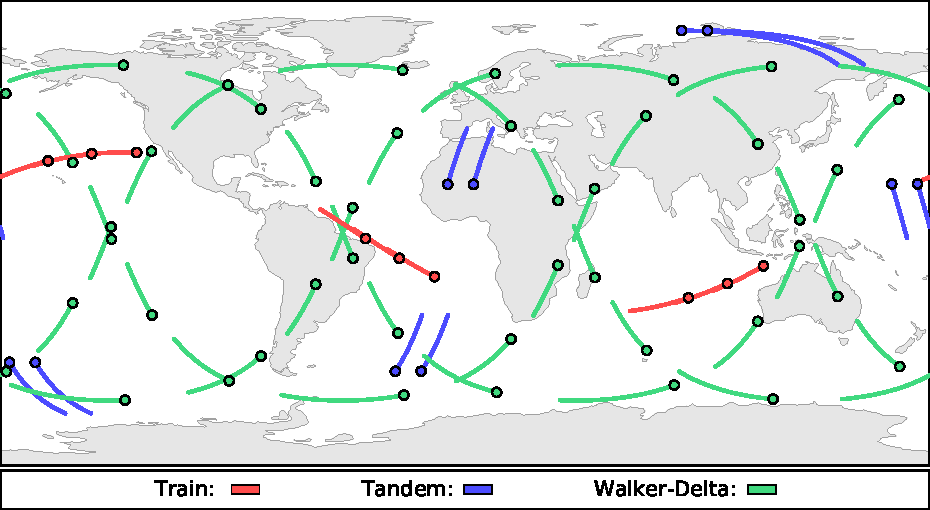
\includegraphics[width=\textwidth]{images/constellations.pdf}
      {\footnotesize(a) Various constellations defined by orbit patterns}
    \end{center}
    \medskip
  \end{minipage}
  \begin{minipage}[b]{\linewidth}
    \begin{center}
      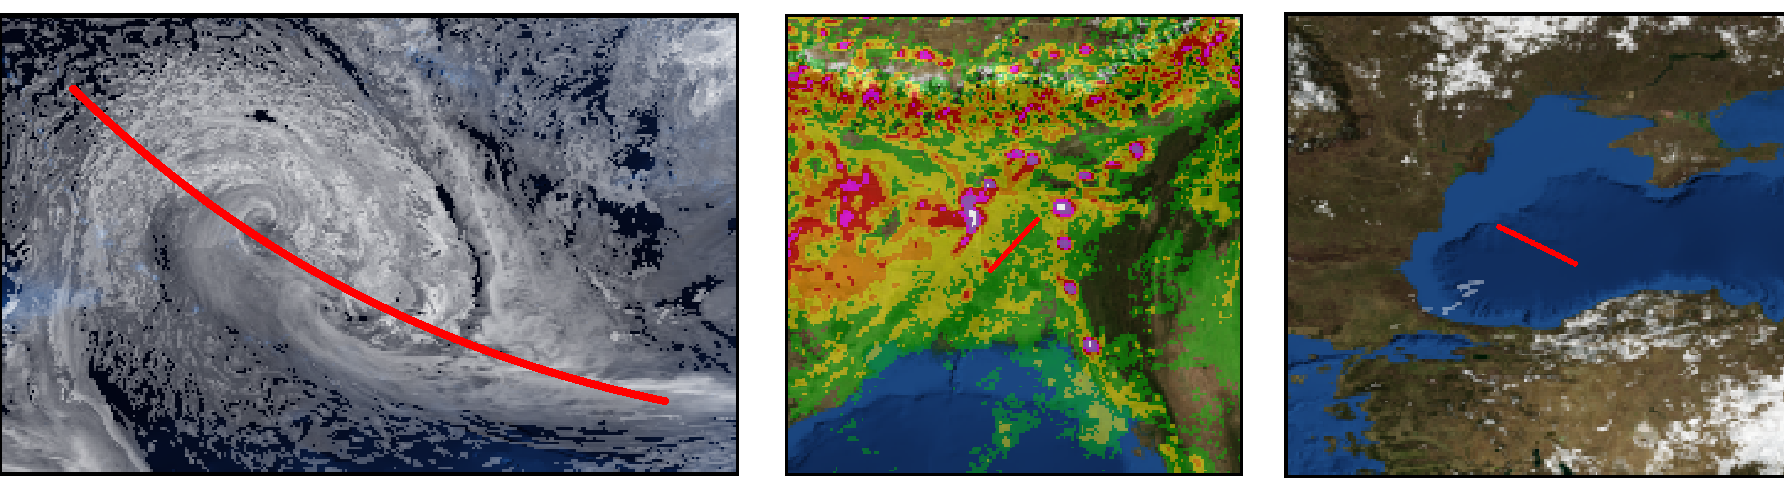
\includegraphics[width=\textwidth]{images/remote_sensing.pdf}
      {\footnotesize{
          \color{white}~~~~~~~~\color{black}
          (b) Cloud Depth~~~~~~~~~~~~
          (c) Precipitation~~~~~
          (d) Optical Images}}
    \end{center}
    \medskip
  \end{minipage}
  \begin{minipage}[b]{\linewidth}
    \begin{center}
      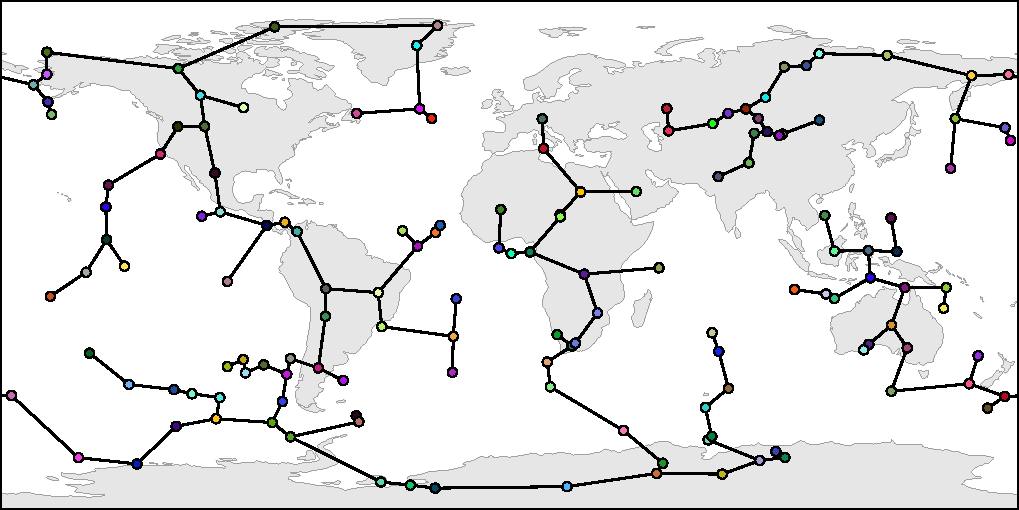
\includegraphics[width=\textwidth]{images/prim.pdf}
      {\footnotesize(e) Instantaneous network graph structure (minimum spanning
        tree)}
    \end{center}
    \medskip
  \end{minipage}
  \begin{minipage}[b]{\linewidth}
    \begin{center}
      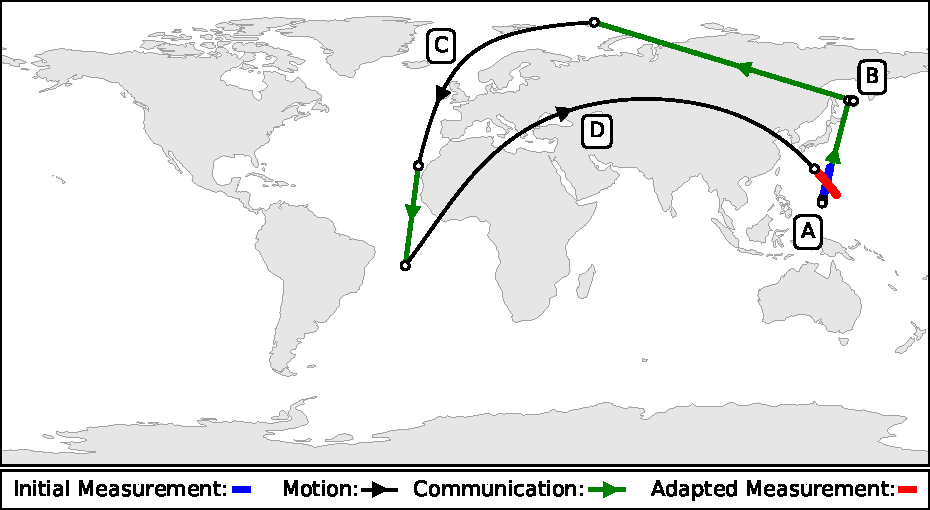
\includegraphics[width=\textwidth]{images/collaborate.pdf}
      {\footnotesize(f) Collaborative sequence in time}
    \end{center}
  \end{minipage}
  \caption{Collaborate software library features}
  \label{fig:features}
\end{figure}

\begin{figure}[t]
  \begin{minipage}[b]{0.49\linewidth}
    \begin{center}
      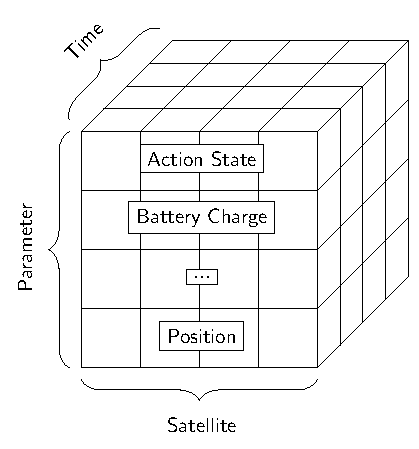
\includegraphics[width=\textwidth]{images/params.pdf}
      {\footnotesize(a) Satellite parameter data}
    \end{center}
  \end{minipage}
  \begin{minipage}[b]{0.49\linewidth}
    \begin{center}
      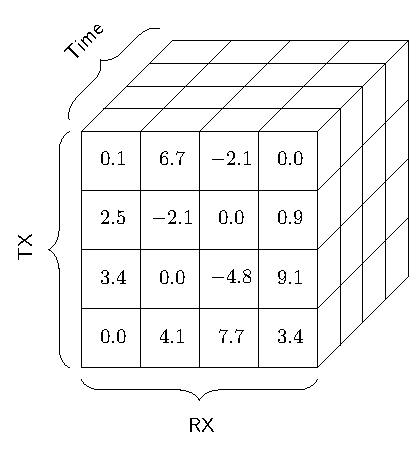
\includegraphics[width=\textwidth]{images/weighted.pdf}
      {\footnotesize(b) Network parameter data}
    \end{center}
  \end{minipage}
  % \newline
  % \begin{minipage}[b]{0.49\linewidth}
  %   \begin{center}
  %     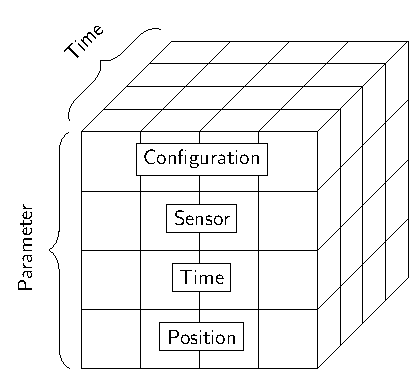
\includegraphics[width=\textwidth]{images/meas2.pdf}
  %     {\footnotesize(c) Satellite measurement data}
  %   \end{center}
  % \end{minipage}
  % \begin{minipage}[b]{0.49\linewidth}
  %   \begin{center}
  %     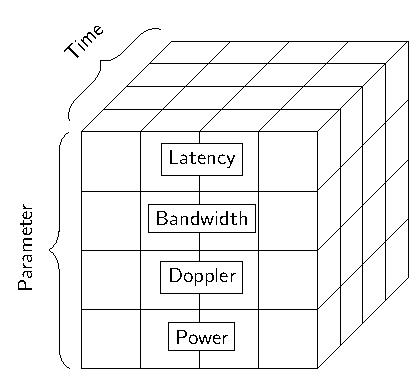
\includegraphics[width=\textwidth]{images/comm.pdf}
  %     {\footnotesize(d) Comm. channel data}
  %   \end{center}
  % \end{minipage}
  \caption{Simulation training data formats}
  \label{fig:data}
\end{figure}

The software logs simulation data to files accessible by external machine
learning tools.  \project was developed around simple data formats for
portability and to promote development of custom analysis tools.  Primarily,
data is serialized and written to binary files.  These formats are well
documented and easy to parse in Python or other scripting languages.  Included
Python packages understand the data formats and can read and store the data for
later use as Numpy or Pandas data structures.  Examples include time-series data
frames or network adjacency matrices (weighted and unweighted).  Fig.2
shows several common data structures in memory.

Python scripts are provided not only for receiving simulation data at a low
level, but also many high level analysis tasks.  In fact, all figures in this
document were produced using the tools provided by the library.  Primary
third-party packages used include the following: Numpy, Pandas, Cython, NetCDF4,
Matplotlib, Cartopy, Scikitlearn, TensorFlow, and SciPy.  These enable post
processing for plots and animations or to train machine learning algorithms.
Numpy and Pandas provide powerful linear algebra and statistics operations.
Cartopy provides extensive map projections and transformations which support
visualizing satellite positions and truth data.  Machine learning algorithms are
available in the Scikitlearn and Tensorflow packages, which interface well with
Numpy and Pandas structures.

For example, satellite parameter data (Fig.2(a)) is plotted in Fig.3(a) to
expose and potentially exploit correlations.  Several of these seem strongly
correlated and many are also periodic.  Potential high-level communications
optimizations may involve predicting when a satellite has the most visible
neighbors (available line-of-sight links).  An algorithm for power management
scheduling may use the instantaneous charge or power to plan efficient sensor
operation.

\begin{figure}[t]
  \begin{minipage}[b]{\linewidth}
    \begin{center}
      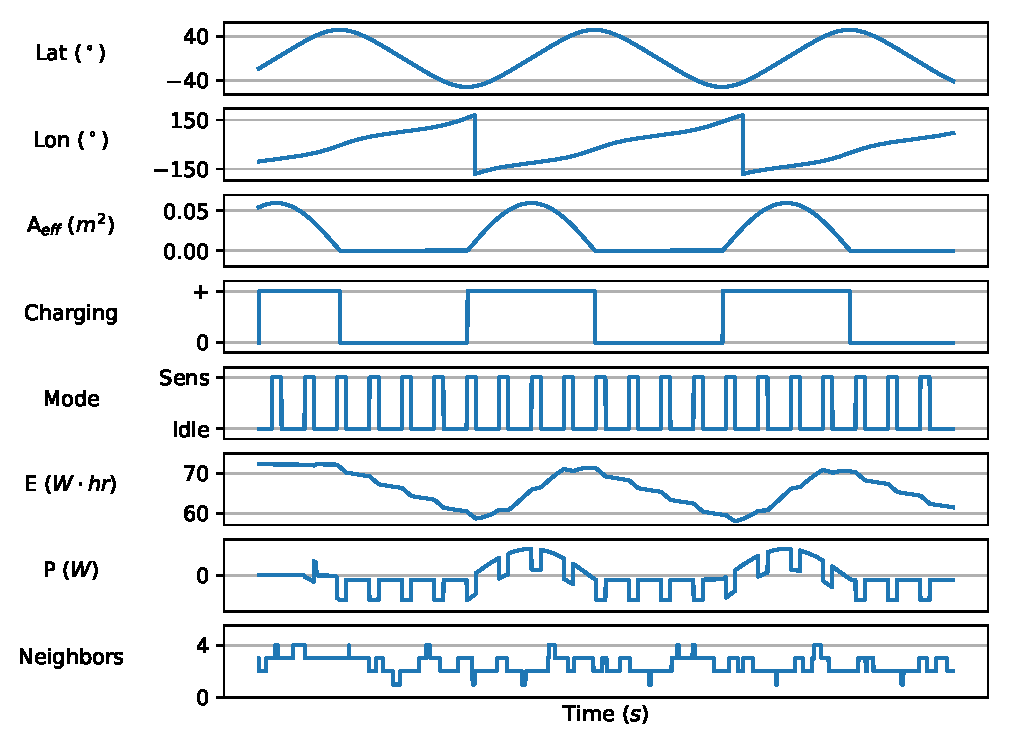
\includegraphics[width=\textwidth]{images/param_plot.pdf} \\
      {\footnotesize(a) Time-series satellite parameters}
    \end{center}
    \medskip
  \end{minipage}
  \begin{minipage}[b]{\linewidth}
    \begin{center}
      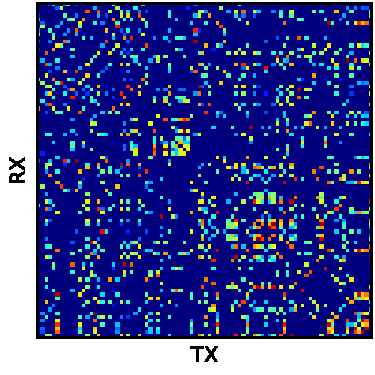
\includegraphics[width=0.5\textwidth]{images/weighted_plot.pdf} \\
      {\footnotesize(b) Instantaneous Line-of-Sight Doppler Adjacency Matrix}
    \end{center}
  \end{minipage}
  \caption{Visualized simulation data}
  \label{fig:processing}
\end{figure}

Another visualization involves network structure.  Fig.3(b) and (c) contain
plots of unweighted and weighted adjacency matrices.  A built-in Python library
called NetworkX produced these graphs and works well with the adjacency matrix
format.

\vspace{80pt}

...

\vspace{80pt}

...

\vspace{80pt}

...

\vspace{80pt}

%% =============================== EXAMPLES ====================================

\section{Example Case Studies}
\label{sec:examples}

The following examples demonstrate cognitive communications and machine learning
techniques applied to software simulations.  First, parametric regression is
automated using the \project network feedback algorithm.  This simulates
deployed machine learning in a realistic observing system.  Second, satellites
are classified based on line-of-sight proximity.  This demonstrates the utility
of \project simulation data for training external machine learning models.

\subsection{Cognitive Feedback For Autonomous Parameter Regression}
\label{ssec:feedback}

One option for increasing an sensor network's operational value is for its
members to make informed decisions about what and when to measure, rather than
using a fixed duty cycle.  Informed decisions would benefit optical imaging
satellites through cloud avoidance or targeting events.  Also, cloud satellites
can exploit data cloud depth correlation to inform follow-up precipitation
measurements.  Section~\ref{sec:software} shows that \project provides a network
algorithm for predicting optimal routes, such as the one illustrated in
Fig.1(f).  This can also be used to predict a path for feedback to the original
satellite.

A single feedback cycle is shown in Fig.4(a).  In this plot, a satellite travels
from South America over the Atlantic and measures cloud depth over Africa (blue
line).  Internal processing reveals the presence of clouds which exceed a
threshold for likely precipitation.  The satellite is able to predict the
arrival of a precipitation sensor.  A message is forwarded through three other
satellites across the Pacific which alerts the follow-up satellite of this
opportunity.  As quickly as possible after the follow-up measurement,
information is fed back to the original satellite over the Middle East and
China.  Feedback provides success or failure criteria, improving the
cloud-sensing satellite's future decisions.



\begin{figure}[t!]
  \begin{minipage}[b]{\linewidth}
    \begin{center}
      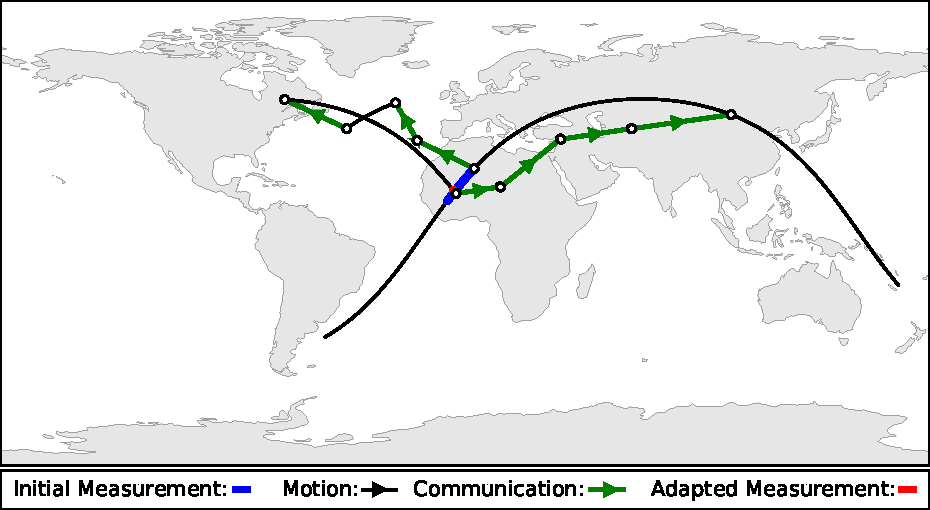
\includegraphics[width=\textwidth]{images/loop.pdf}
      {\footnotesize(a) Feedback route}
    \end{center}
    \medskip
  \end{minipage}
  \begin{minipage}[b]{\linewidth}
    \begin{center}
      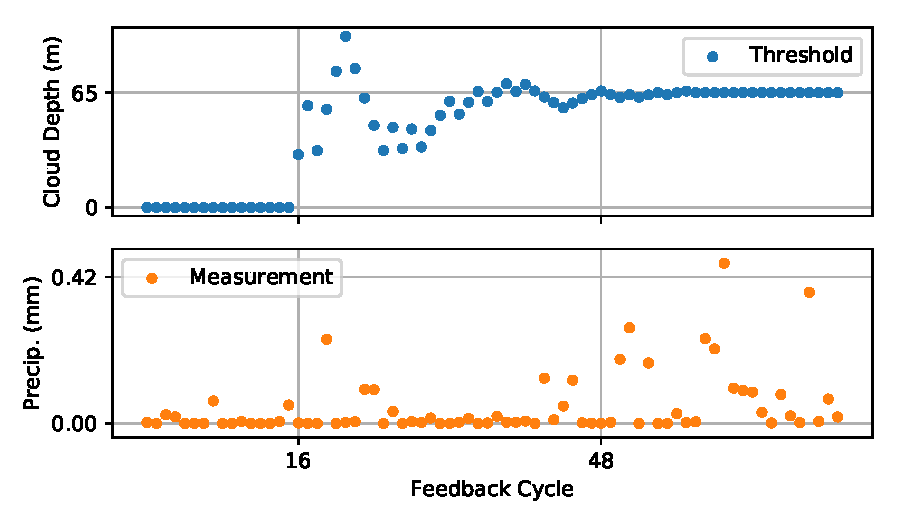
\includegraphics[width=\textwidth]{images/regression.pdf}
      {\footnotesize(b) Autonomous parametric regression for data correlation
        threshold}
    \end{center}
  \end{minipage}
  \caption{Cognitive communications feedback}
  \label{fig:feedback}
\end{figure}

\subsection{Spectral Clustering Using Simulated Network Data}
\label{ssec:cluster}

\begin{figure}[t!]
  \centerline{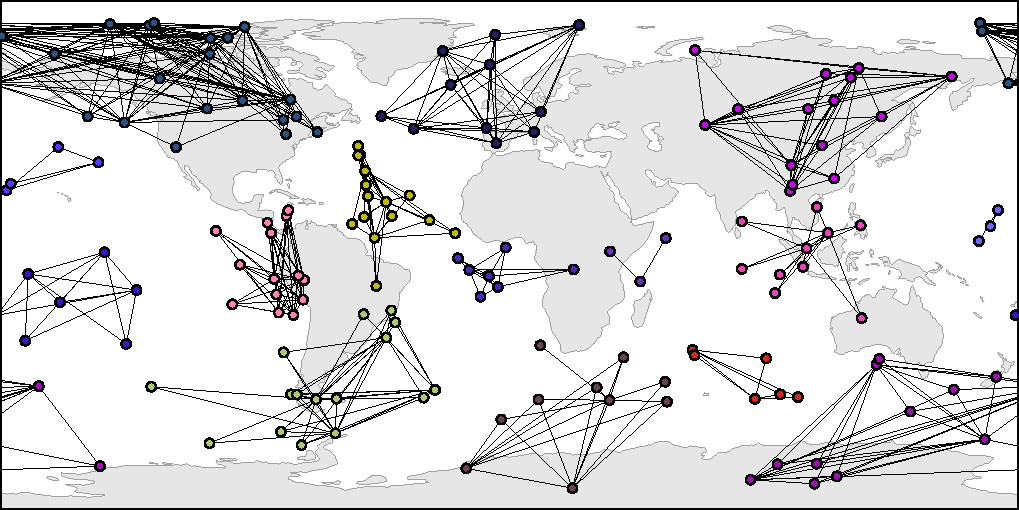
\includegraphics[width=\linewidth]{images/clusters.pdf}}
  \caption{Spectral clustering by k-means classification}
  \label{fig:clusters}
\end{figure}

\vspace{80pt}

...

\vspace{80pt}

...

\vspace{80pt}

...

\vspace{80pt}

...

\vspace{80pt}

%% ================================ SUMMARY ====================================

\section{Summary And Next Steps}
\label{sec:summary}

\vspace{80pt}

%% =============================== REFERENCES ==================================

\begin{thebibliography}{9}
{\small
\bibitem{ref1} Paper on NASA vision statement for small satellite constellations
\bibitem{ref2} Paper on data volume issues with small satellties.  Need for onboard processing
\bibitem{ref3} Paper on overview of cognitive communications for satellites (probably CCAA paper)
\bibitem{ref4} Paper on low-level of cognitive communications for satellites (probably CCAA paper)
\bibitem{ref5} Paper on low-level of cognitive communications for satellites (probably CCAA paper)
\bibitem{ref6} R. Linnabary, IGARSS paper reference

\bibitem{refx} G. E. Smith, A. E. Mitchell, C. D. Ball, A. O'Brien, and J. T. Johnson, ``Fully adaptive remote sensing observing system simulation experiments'', in {\it Proceedings of the IEEE International Geoscience and Remote Sensing Symposium (IGARSS)}, July 2018, pp. 5839-5842.
}
\end{thebibliography}

\end{document}
